%%%%%%%
% Ch1       %
%%%%%%%

\chapter{Introduction}
	
	\begin{center}
		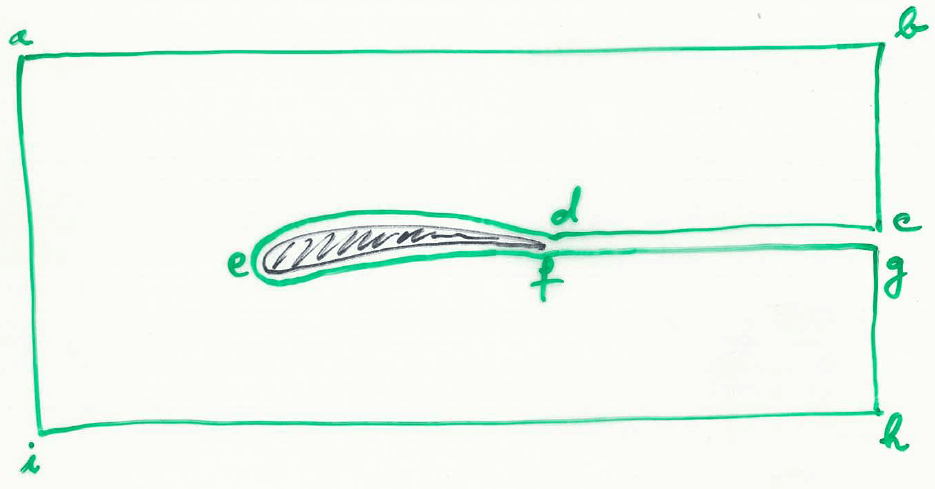
\includegraphics[scale=0.65]{ch1/1}
		\captionof{table}{List of abbreviations and symbols.}
		\label{table:1.1}
	\end{center}
	
	In the previous page, there's a table with abbreviations and symbols used in this chapter.
	The difference between power electronics and signal electronics is the high power consumption. We will focus on the conversion from one form of energy to another and not on signal transmission and analysis. In this course, we will study converters working at steady state. The distortion of physical quantities will be a nuisance.
	
\section{Different types of converters, semi-conducting components and applications}
	\subsection{Types of converters}
		Power electronics converters change properties of the electric energy between the input and the output. The different kinds of conversions and the corresponding converters relevant to this course are in \autoref{table:1.2}.
		
		We should remark the fact that converters are reversible when it comes to power, that is to say electric power can flow from the input to the output and conversely. The choice of the input will therefore depend on the main direction of the power flux for a given converter or application. This property is natural for electromagnetic converters (e.g. transformers) but it is not respected by static converters. This kind of converters contain semi-conducting components, which are non-linear, as well as magnetic components and capacitors.
		

		\begin{center}
			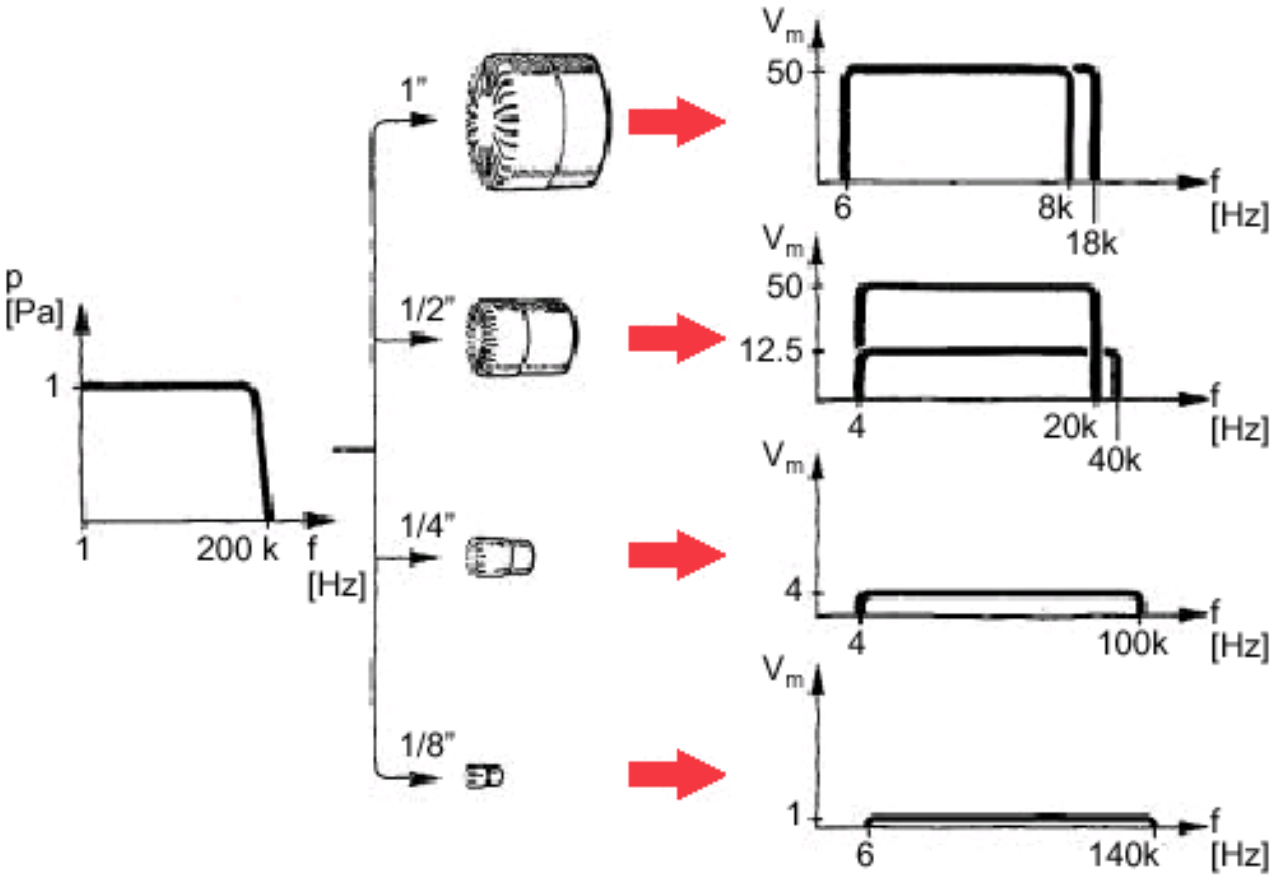
\includegraphics[scale=0.5]{ch1/2}
			\captionof{table}{Types de convertisseurs.}
			\label{table:1.2}
		\end{center}
		
	\subsection{Types of semi-conducting components}
	    We can classify the semi-conducting components according to their controllability: 

		\begin{itemize}
			\item[•] \textbf{Diodes} are non-linear and uncontrollable components. They are equivalent to a short-circuit following one direction and to an open circuit following the other direction. \textbf{Uncontrolled rectifiers} composed of diodes are widely employed. \\
			Frequency capacity: small to big.
			Power capacity: small to big.\\
			
			\item[•] \textbf{Thyristors} hold multiple diodes and a control electrode which allows the delay of the conduction but not the stop of the current. That is why they are called \textbf{semi-controllable.}  With \textbf{thyristor rectifiers}, we can control the output voltage and we can inverse it as well. They are also present in \textbf{AC choppers} and \textbf{cycloconverters}. Thyristors are \textbf{unidirectional} when it comes to current as diodes are.\\
			Frequency capacity: small.
			Power capacity: big.\\
			
			\item[•] The  \textbf{triac} is very similar to the thyristor because it is \textbf{semi-controllable}. However, it is \textbf{bidirectional} for the current too. That is because of the presence of two thyristors set in anti-parallel. We use them to compose \textbf{AC choppers}.\\
			Frequency capacity: small.
			Power capacity: small.\\
			
			\item[•] The last category of semi-conducting components comprises the fully controllable components. They are the \textbf{power transistors} (BJT, IGBT, MOSFET, ...) and components derived from the thyristor (GTO). We also call them \textbf{controllable switches}. They can be found in \textbf{universal bridges}. We call them universal because they can effect various energy conversions. \\
			In the order GTO - BJT, IGBT, ... - MOSFET, frequency capacity: small - medium - big, power capacity: big - medium - small. 
		\end{itemize}
		
	\subsection{Types of applications}
		\begin{wrapfigure}[9]{l}{3.7cm}
		\vspace{-5mm}
		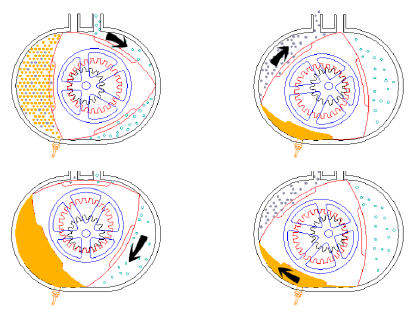
\includegraphics[scale=0.25]{ch1/4}
		\captionof{figure}{}
		\end{wrapfigure}	
		The AC-AC conversion is widely employed, in particular for the supply and control of AC electric machines. AC choppers and cycloconverters do this in only one step but they are very limited. The concatenation of an AC-DC converter and a DC-AC converter, with a capacitor (in parallel) or a self (in series) between them working as an energy limiter, will give more flexibility. We do the same thing for a DC machine by using a DC-DC converter instead of the DC-AC converter.
		
		\ \\
		\begin{wrapfigure}[8]{r}{3.5cm}
		\vspace{0mm}
		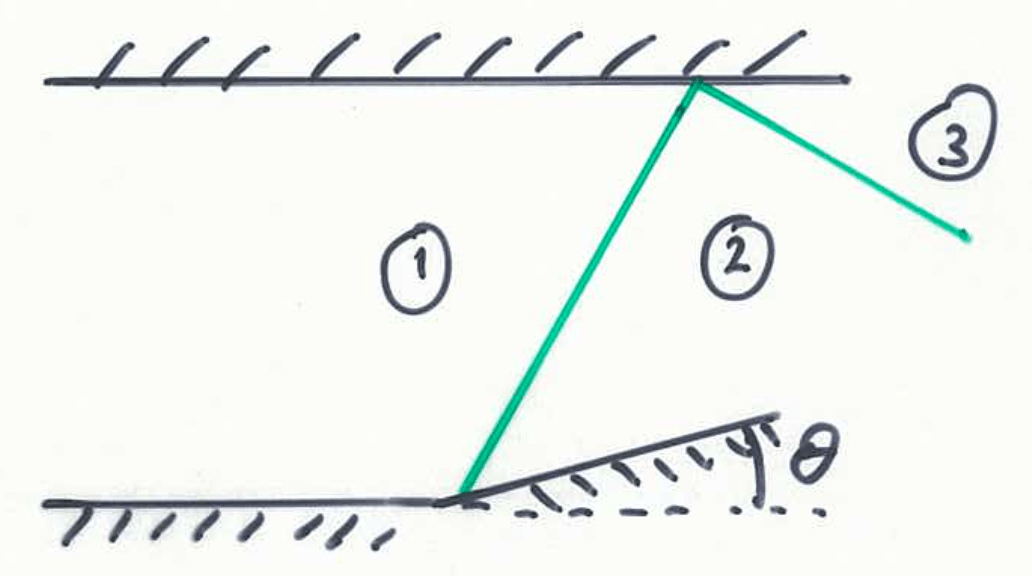
\includegraphics[scale=0.25]{ch1/5}
		\captionof{figure}{}
		\end{wrapfigure}
		
		A converter can be plugged into the grid if we put a transformer as an intermediary step. Depending on the type of converter and the load, a current more or less distorted is obtained as a result. As the supply has an inner impedance, the distorted voltage appear at the PCC (Point of Common Coupling). That might induce problems and damages in the other loads. That happens when the load has a bad \textbf{electromagnetic compatibility} (EMC). The problem of harmonics can be fixed by using \textbf{passive filters} (capacitors and inductors) or \textbf{active filters} (controllable converters).\\
		
		Another relevant aspect is the \textbf{reactive power} of the network (AC network) and/or of the load (AC load). Some converters can supply reactive power instead of pulling a current retarded with respect to the voltage. This is crucial for asynchronous machines working as loads because they consume reactive power. The reversibility of the active power consumption of the converter is equally important. For example, the recovery of electric power from the braking or its dissipation in a resistance. 
		

\section{Periodic regimes and harmonics}
	\begin{wrapfigure}[6]{l}{5cm}
	\vspace{-5mm}
	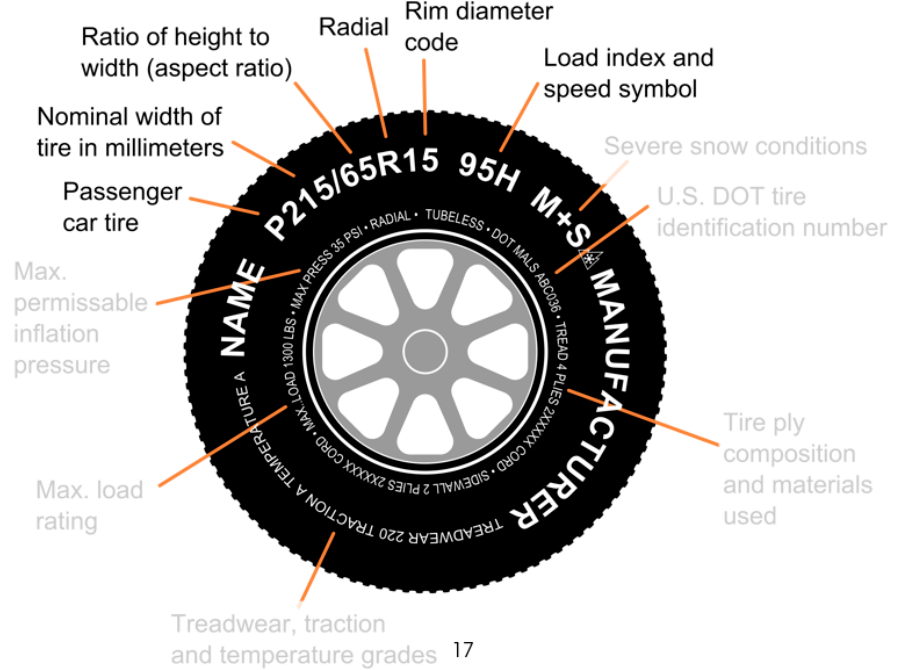
\includegraphics[scale=0.25]{ch1/6}
	\captionof{figure}{}
	\end{wrapfigure}
	
	In this course, when studying converters we will focus on steady-state operating conditions. Currents and voltages are therefore periodic functions where the fundamental period is designed by $T$. In the figure, the first signal can be designed as continuous because it remains positive and the continuous component is dominating whereas the second one is considered as an alternative signal even if it has a continuous component. The peak-to-peak ripple is the difference between the maximum and the minimum value of the signal. The fundamental frequency $f = 1/T$ is directly linked to the frequency of the power supplied to the converter, or to the controlled cutting frequency. The presence of non-linear components and the cutting of the switches distort the signals.

		
	\subsection{Fourier analysis}
	If we consider a periodic function $i(t)$ whose fundamental pulsation is $\omega = 2\pi f = 2\pi /T$, its decomposition is given by:

	\begin{equation}
	\begin{aligned}
		i(t) &= I_0 + \sum _{k\geq 1} \left(Î_{ck} \cos k\omega t + Î_{sk} \sin k\omega t\right)\\
			&= I_0 + \sum _{k\geq 1} \underbrace{Î_k \cos (k\omega t +\gamma _k)}_{i_k(t)} \qquad with \qquad Î_{ck} - jÎ_{sk} = Î_k e^{j\gamma _k},
	\end{aligned}
	\end{equation}
	where $I_0$ is the continuous component and $i_k(t)$ is the rms value of harmonic of order k. The continuous component gives the average value of $i(t)$ over a fundamental period because the average value of each harmonic is equal to zero: 
	\begin{equation}
		I_0 = \frac{1}{T}\int _0 ^T i(t)\, dt
	\end{equation}
	The orthogonality equation from page 7 of the syllabus furnishes the following relations for $k\geq 1$ : 
	\begin{equation}
	\begin{aligned}
		Î_{ck} &= &Î_k \cos \gamma _k &= \frac{2}{T} \int _0 ^T i(t) \cos k\omega t\, dt\\
		Î_{sk} &= &-Î_k \sin \gamma _k &= \frac{2}{T} \int _0 ^T i(t) \sin k\omega t\, dt
	\end{aligned}
	\end{equation}
	
	The \textbf{half-wave symmetry} manifests itself very often in practical cases. By definition there is half-wave symmetry when $v(t) = -v(t+T/2)$ or $i(t) = -i(t+T/2)$. This allows us to neutralize even-order harmonics: 
	\begin{equation}
		\int _0 ^T v(t)\cos k \omega t \, dt = \frac{1}{T}\int _0 ^{T/2} v(t) \underbrace{\left(\cos k\omega t - \cos k\omega(t+T/2)\right)}_{\mbox{= 0 if k is even}}\, dt
	\end{equation}
	
	\subsection{Root-mean-square (rms) value}
		The rms value of the current $i(t)$ is given by:
		\begin{equation}
			I_{rms} = \sqrt{\int _0 ^T i^2(t) \, dt} = \sqrt{I_0^2 + \frac{1}{2}\sum _{k\geq 1}Î_k ^2 } = \sqrt{I_0^2 + \sum _{k\geq 1} I_k^2},
		\end{equation}
		where $I_k = \frac{1}{\sqrt{2}}Î_k$ is the rms value of harmonic of order $k$. The product of harmonic components of different orders $I_kI_l$ doesn't appear because of their orthogonality. If we consider the current flowing through a resistance $R$, the \textbf{Joule losses} are $Ri^2(t)$ and the \textbf{average power over a fundamental period T} is given by:
		\begin{equation}
			P_J = \frac{1}{T}\int _0^T Ri^2 \, dt = RI_0^2 + \sum _{k\geq 1} RI_k^2 = RI_{rms}^2,
		\end{equation}
		and they are therefore proportional to the square of the rms value of the current.

		
	\subsection{Instantaneous and average electrical power}
	    If we consider a voltage $v(t)$ and a current $i(t)$, both periodic of period T:
		\begin{equation}
			v(t) = V_0 + \sum _{k \geq 1} \underbrace{\sqrt{2} V_k \cos (k\omega t+ \gamma _{vk})}_{v_k(t)} \qquad and \qquad
			i(t) = I_0 + \sum _{k \geq 1} \underbrace{\sqrt{2} I_k \cos (k\omega t+ \gamma _{ik})}_{i_k(t)}
		\end{equation}
		The instantaneous power associated to them is given by $p(t) = v(t)i(t)$ and the average power
		\begin{equation}
			P = \frac{1}{T}\int _0 ^T p(t)\, dt = \underbrace{V_0I_0}_{P_0} + \underbrace{V_1I_1\cos \varphi _1}_{P_1} + \sum _{k\geq 2}\underbrace{V_kI_k \cos \varphi _k}_{P_k}
			\label{eq:1.8}
		\end{equation}
		where $P_0$ is the power associated to the continuous component, $P_k$ to the harmonic of order $k\geq 1$ and where $\varphi _k = \gamma _{vk} - \gamma _{ik}$ is the phase lag angle of current with respect to voltage (order k). Once again the product of different order of harmonics doesn't appear. The addition in \eqref{eq:1.8} can be limited to a single term:
		\begin{itemize}
			\item[•] If the voltage $v(t)$ is continuous and not distorted ($v(t) = V_0; V_k = 0, k\geq 1$) the average power is given by $P = V_0I_0$ for any possible current. The same happens when we inverse current and voltage. 
		 
			\item[•] If the voltage is sinusoidal and not distorted ($v(t) = \sqrt{2}V_1\cos (\omega t + \gamma _v); V_k = 0, k\neq 1$), the average power is given by $P = V_1I_1\cos \varphi _1$ for any possible current. The same happens when we inverse current and voltage. 
			
		\end{itemize}
		Anyways, $P_k$ often remains negligible with respect to $P_0$ or $P_1$. 
		
	\subsection{DC quantities}
	In absence of distortion, the DC quantities are constant. The distortion of the current $\Delta i(t)$ can comprise all the harmonics of order $k\geq 1$ : 
		\begin{equation}
			i(t) = I_0 + \underbrace{\sum _{k\geq 1} Î_k \cos (k\omega t +\gamma _k)}_{\Delta i(t)}
		\end{equation}
		The rms value of the distortion $\Delta i(t)$ is given by: 
		\begin{equation}
			\Delta I_{rms} = \sqrt{\frac{1}{2}\sum _{k\geq 1} Î_k^2} = \sqrt{\sum _{k\geq 1} I_k^2}
		\end{equation}
		The rms value of the current can therefore be written differently: 
		\begin{equation}
			I_{rms} = \sqrt{I_0^2+\Delta I^2_{rms}}.
		\end{equation}
		The supplementary Joule losses induced by the distortion are given by $R(\Delta I_{rms})^2$. 
		
	\subsection{Sinusoidal quantities (single phase systems)}
	    When there's no distortion, the AC quantities are perfectly sinusoidal. The distortion, if there's any, manifests itself as a continuous component $I_0$ and harmonics of order $k\geq 2$ :
		\begin{equation}
			i(t) = \underbrace{Î_1\cos (\omega t+\gamma _1)}_{i_1(t)} + \underbrace{I_0 + \sum _ {k\geq 2} Î_k \cos (k\omega t + \gamma _k)}_{\Delta i(t)}
		\end{equation}
		The rms value of the distortion is given by: 
		\begin{equation}
			\Delta I_{rms} = \sqrt{I_0^2+\frac{1}{2}\sum _{k\geq 2} Î_k^2} = \sqrt{I_0^2+ \sum _{k\geq 2} I_k^2}
		\end{equation}
		The \textbf{THD - Total Harmonic Distortion} of an AC quantity is defined as the ratio of the rms value of the distortion and the rms value of the fundamental component:
		\begin{equation}
			THD = \frac{\Delta I_{rms}}{I_1}
		\end{equation}
		The \textbf{DPF - Displacement Power Factor} is defined as the cosine of the angle $\varphi _1$ (the phase lag angle of the fundamental component of the current w.r.t. the fundamental component of the voltage): 
		\begin{equation}
			DPF = \cos \varphi _1.
		\end{equation}
		The \textbf{apparent power S} and the \textbf{PF - Power Factor} are defined as:
		\begin{equation}
			S = V_{rms}I_{rms} \qquad and \qquad PF = \frac{P1}{S} = \frac{V_1I_1\cos \varphi _1}{V_{rms}I_{rms}}
		\end{equation}
		where $P_1$ is the average (or active) power associated with fundamental harmonics. The PF is almost always smaller to 1 because of the phase lag $\varphi _1$ or the distortion of either the voltage or the current ($V_{rms}>V_1$ or $I_{rms}>I_1$). For AC power transmission, a load is considered ideal if, when it is plugged into a perfect sinusoidal voltage source, the absorbed current is perfectly sinusoidal, the resistance is constant and there's no phase shift. When this happens the DPF and the PF are equal to 1. The Joule losses and the rms value of the current are minimal when that happens. 
		
		\subsubsection{Square-wave and triangular current}
			\begin{center}
			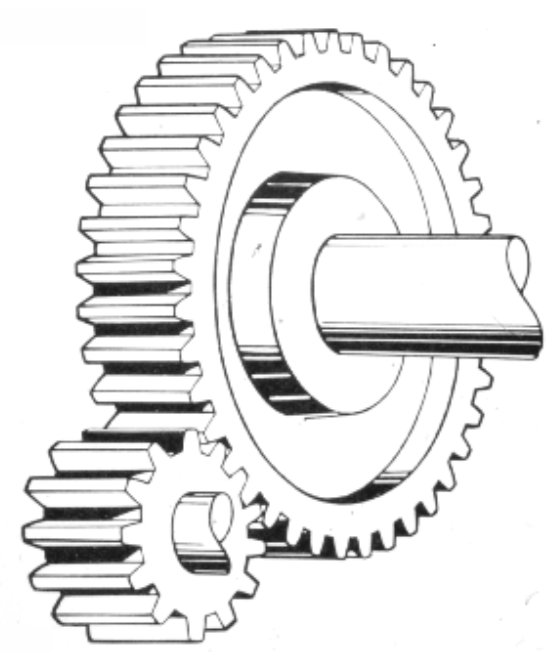
\includegraphics[scale=0.4]{ch1/7}
			\captionof{figure}{}
			\end{center}
			According to the figure, the square-wave voltage $v(t)$ fluctuates between $\hat{V}$ and $-\hat{V}$. The amplitude and the rms value of the fundamental period are given by: 
			\begin{equation}
				\hat{V}_1 = \frac{4}{\pi}\hat{V} \qquad and \qquad V_1 = \frac{2\sqrt{2}}{\pi} \hat{V}
			\end{equation}
			As even order harmonics are absent of the spectre because of the half-wave symmetry and the amplitude of harmonic of order $k\geq 1$ is inversely proportional to their order $\hat{V}_k = \frac{1}{k}\hat{V}_1$: 
		   	\begin{equation}
		   		THD = \sqrt{1/3^2 + 1/5^2+1/7^2+ \dots} = 48.3\%
		   	\end{equation}
			In order to obtain a \textbf{triangular current}, we impose a square-wave voltage $v(t) = \pm \hat{V}$ to a self of inductance L. As a result, we obtain a triangular current of gradient $\frac{di}{dt}= \pm \frac{1}{L}\hat{V}$. The half-wave symmetry appears in this wave too and the odd order harmonics are linked together as follows:
		   	\begin{equation}
		   		\hat{V}_k \cos (k\omega t+ \gamma _k) = L\frac{d}{dt}\left( Î_k \sin (k\omega t+ \gamma _k)\right)\qquad \Rightarrow  \hat{V}_k = k\omega L Î_k
			\end{equation}		  
			Therefore, the amplitude of harmonics of odd orders $k\geq 1$ are $Î_k = \frac{1}{k^2}Î_1$. The current is less distorted than the voltage:
			\begin{equation}
				THD = \sqrt{1/3^4+1/5^4+1/7^4+\dots} = 12.12\%
			\end{equation}
			We can study the analogous case by imposing the flow of a square wave current through a capacitor. The slope of the triangular voltage is given by $\frac{dv}{dt} = \pm \frac{1}{C}Î$ and the harmonics are linked together as follows: 
		   	\begin{equation}
		   		Î_k = k\omega C \hat{V}_k.
		   	\end{equation}
		   	
	\subsection{Three-phase square-wave}
		\subsubsection{Arbitrary periodic regime}
		Let's consider 3 currents $i_a(t)$, $i_b(t)$ and $i_c(t)$, with the same fundamental period T. That's a three-phase system if three quantities are equal but they have a shift equal to $\pm T/3$, for \textbf{direct phase order} and \textbf{inverse phase order} that means:
		\begin{equation}
			i_a(t) = i_a(t+T/3) = i_a(t-T/3) \qquad and \qquad i_a(t) = i_a(t-T/3) = i_a(t+T/3)
		\end{equation}
		
		The signal is called \textbf{homopolar} when all the currents are identical. When it comes to \textbf{harmonic content}, for a direct order system with half wave symmetry (no even harmonics), the order $k$ of the remaining harmonics can be written as $k = 6m+1, k = 6m +3, k= 6m+5$ ($n \in Natural$ numbers). The expressions of the currents are developed as follows: 
		\begin{equation}
			i_a(t) = \sum _{k = 6m+1}Î_{a,k} \cos (k\omega t + \gamma _{a,k})+ \sum _{6m+3}Î_{a,k} \cos (k\omega t + \gamma _{a,k}) + \sum _{6m+5}Î_{a,k} \cos (k\omega t + \gamma _{a,k})
		\end{equation}
		
		Symmetry is also of application for harmonics, then the amplitude of the current is the same for all the phases. In order to find the relation between the phase angles we will exploit the direct phase order properties:
			\begin{equation}
				\cos (\omega t + \gamma _{a,k}) = \cos (\omega t + \gamma _{b,k} + \frac{2\pi}{3}) = \cos (\omega t + \gamma _{c,k} - \frac{2\pi}{3}). 
			\end{equation}
			\begin{itemize}
				\item[•] If $k = 6m+1 :$\\
				We obtain $\gamma _{a,k} = \gamma _{b,k} + \frac{2\pi}{3} = \gamma _{c,k} - \frac{2\pi}{3}$. The harmonics form a direct phase order three-phase system of period $T/k$. 
				\item[•] If $ k = 6m+3 :$\\
				We obtain $\gamma _{a,k} = \gamma _{b,k} = \gamma _{c,k}$. This corresponds to homopolar systems $k = 3, 9, ...$.when the addition of the phases equals 0 at any time, $i_{a,k}(t)+i_{b,k}(t)+i_{c,k}(t) = 0$. Harmonics multiples of 3 are therefore eliminated. 
				\item[•] If $k = 6m+5$\\
				We obtain $\gamma _{a,k} = \gamma _{b,k} -\frac{2\pi}{3} =\gamma _{c,k}+\frac{2\pi}{3}$. These harmonics correspond to inverse phase order three-phase systems. 
				 \newpage
			\end{itemize}
			
		\subsubsection{Three phase square wave}
			\begin{wrapfigure}[9]{l}{4cm}
			\vspace{-5mm}
			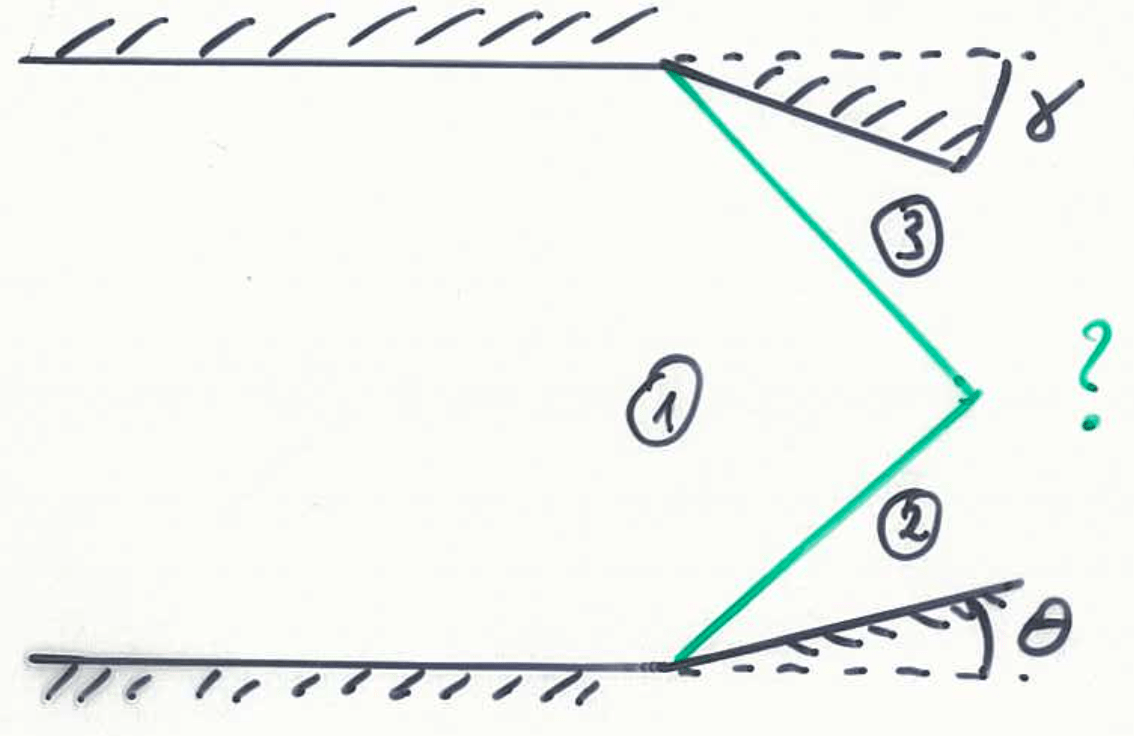
\includegraphics[scale=0.20]{ch1/8}
			\captionof{figure}{}
			\end{wrapfigure}		
			In the figure we observe easily the direct order symmetry existent between the currents (of fundamental period $T$). The impulsions of period $T/3$ are separated by intervals of length $T/6$. The amplitude and the rms value of the current are given by:
			\begin{equation}
				Î_{1} = \frac{2\sqrt{3}}{\pi} Î \qquad and \qquad I_1 = \frac{\sqrt{6}}{\pi} Î.
			\end{equation}
			There's only odd order harmonics (half-wave symmetry) and harmonics of orders divisible by 3 are also excluded (homopolar components). The components of the current are $Î _k = Î_1/k$ and the THD is:
			\begin{equation}
				THD = \sqrt{1/5^2 + 1/7^2 + 1/11^2 / \dots} = 31.1\%
			\end{equation}
			
	\subsection{Zero average voltage across an inductance and zero average current in a capacitor}
		\subsubsection{Inductance}
		If the signal is at steady state and has a period $T$, the average voltage $V_{L,0}$ equals 0 (for a constant inductance) :
			\begin{equation}
				V_{L,0} = \frac{1}{T}\int _{t_0}^{t_0+T} v_L (t)\, dt = \frac{L}{T}\int _{t_0}^{t_0+T} \frac{di_L}{dt}\, dt = \frac{L}{T}\left(i_L(t_0 + T) - i_L(t_0)\right) = 0
			\end{equation}
		The same thing happens in the case of a non linear inductance if we are in steady state because the flux is periodic $\phi _L(T+t_0) = \phi _L (t_0)$ and $v_L = \frac{d\phi _L}{dt}$. In steady state, the inductance absorbs and debits magnetic energy alternatively according to the expression $e_L(t) = \frac{1}{2} Li_L^2$. The current fluctuates around its average value $I_{L,0}$ and the energy fluctuates around $E_{L,0}=\frac{1}{2} L I_{L,rms}^2$ at twice the fundamental frequency. 
			
		\subsubsection{Capacitor}
		At steady state, a periodic signal of period $T$ has an average current equal to 0 for a constant capacity $C$ : 
		\begin{equation}
			I_{C,0} = \frac{C}{T}\int _{t_0}^{t_0+T} \frac{dv_C}{dt} \, dt = \frac{C}{T} (v_{C}(t_0+T)-v_C(t_0)) = 0
		\end{equation}
		
		The electric energy collected between the electrodes of the capacitor is $e_C(t) = \frac{1}{2}Cv^2_C$. It debits and absorbs power alternatively, where the voltage oscillates around $V_{C,0}$ while the energy oscillates around $E_{C,0} = \frac{1}{2} C V_{C,rms}^2$. 